\documentclass[	%----------------------Preamble---------------------------------------------------%
		11pt,a4paper,	% fontsize and papersize
		twoside,		% double sided layout
		english,		% document language (also numberingsystem)
		%ngerman,		% document language (also numberingsystem)
		f1				% HsH facultie (f1-f5)
	]{HsH-report}		% documentclass

\usepackage{color}		% for colouring stuff
\usepackage{siunitx}	% units
\usepackage{listings}
\usepackage{csvsimple}	% for importing CSV files
\usepackage{subfigure}	% for subfigures
\usepackage{biblatex}	% bibliography
\usepackage{soul}		% strikethrough text
\usepackage{amssymb}	% spacial Math symbols
\addbibresource{src/localBibliography.bib}


\usepackage{lipsum}		% dummy text
\begin{document}

\pagenumbering{Roman}	% different numbering until first chapter
\maketitle				% using personal.tex
\declarationAuthorship

\begin{abstract}
	\lipsum[5-8]
\end{abstract}

\tableofcontents

\cleardoublepage % important when using double sided layout
\pagenumbering{arabic} % numbering in normal numbers

\chapter{Examples}
	\label{chap: one}
	{\color{red}red text} and {\color{blue}blue text} \\
	different subscripts: \normalsubscripts$R_t$ \upsubscripts$R_t$ \\
	using Units: $R=200\,\milli\ohm + \SI{0.34567453}{\volt\per\metre} - 5\,\si{\second\per\metre\squared}$ \\
	some information\cite{laboranleitung:physik}\\
	german number: $3,5$ english number: $3.5$\\ % note changes when using ngerman document option

	\section{using images}
	Images can just be imported and used in a float environment with a caption and a lable to reference it.
	\begin{figure}
		
\includegraphics[width=.6\textwidth]{img/lorem-ipsum.jpg}
		\caption{just a random image}
	\end{figure}

	Plots can be created directly with latex. It is recommended to do this in subfiles and just import the finished PDF pages. This speed us
	compilertimes by a lot. You should not change the size of precompiled images to keep fontsizes consistent.
	\pagebreak
	\begin{figure}
		\includegraphics[page=2]{plt/build/examplePlot.pdf}
		\caption[centering]{a nice plot}
		\label{fig: plot1}
	\end{figure}
	\begin{figure}
		\includegraphics[page=1]{plt/build/examplePlot.pdf}
		\caption{a area plot}
		\label{fig: area}
	\end{figure}

	Circuit diagramms can also be created using a package called \lstinline{circuitikz}. It is also recommended to get familiar with Inkscape which
	has a very good export to latex feature.
	\begin{figure}
		\graphicspath{{svg/build/}} % double curly brackets needed for unknown reason
		\subfigure[a circuit diagramm]{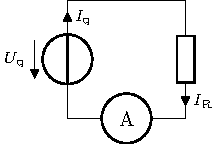
\includegraphics{crc/build/exampleCircuit.pdf}}
		\hspace{2cm}
		\subfigure[made via Inkscape]{\input{svg/build/exampleSVG.pdf_tex}}
		\caption{using two figures}
	\end{figure}

\section{demo nested listing}
	\begin{itemize}
		\item hallo
		\begin{itemize}
			\item temp
			\begin{itemize}
				\item temp
				\begin{itemize}
					\item temp
				\end{itemize}
			\end{itemize}
		\end{itemize}
	\end{itemize}


\section{using Units}
	For this the \lstinline{siunitx} package is used. It provides Macros for all units.
	\begin{equation}
		200\,\kg
	\end{equation}
	The space between a number and it's unit should be a protected half-space, which can be created in latex using \lstinline{\,} In the classfile
	siunits is set up to use a separate macro for each subunit, even for size-modifiers:
	\begin{equation}
		200\,\milli\metre \cdot 2\,\mega\volt
	\end{equation}
	Siunits also allows for reformatting of numbers as well as units. Use the \lstinline{\SI} and \lstinline{\si} macros for that:
	\begin{equation}
		e = \SI{1.602176634E-19}{\coulomb} % formats number + units, autospacing, transform to german comma
		\;|\; \SI[exponent-to-prefix]{2e-9}{\farad} % you can also autocalculate prefixes
	\end{equation}
	\begin{equation}
		\SI[exponent-to-prefix]{1e-6}{\metre}
	\end{equation}
	\begin{equation}
		124\,\si[per-mode=fraction]{\kilo\metre\per\second\squared} % only units
	\end{equation}
	\begin{equation}
		\num{0.0004}\,\lumen % only numbers,  \per and \squared do not work
	\end{equation}

\section{Using formulas}
	\label{sec: formula}
	a numberd formula:
	\begin{equation}
		\label{eq: einhalb} % always lable your stuff
		0,5=\frac{1}{3}
	\end{equation}
	\autoref{eq: einhalb} is nice, but how about multiple lines:
	\begin{equation}
	\begin{split} % you need do nest this
		x &= x^2+3 \\
		\Leftrightarrow 0 &= x^2-x+3 \\
	\end{split}
	\end{equation}
	and how could you align formulas?
	\begin{align}
		x_1 &= 6 &&|\;\mbox{mit } x \in \mathbb{N} \\
		x_2 &= 33+\abs{\frac{1}{4}} &&|\;x_1+3 \\
			&= 33,25 &&\mbox{| don't number everything} \notag \\
		x_3 &= 10^{22}
	\end{align}

\section{formating code}
	\label{sec: code}
	use the listings package:
	% how to skip fist tab??
	\begin{lstlisting}[language=c]
	#include <stdlib.h>
	#include <sdtio.h>

	int main(void) {
		printf("Hello World");
		return 0;
	}
	\end{lstlisting}
	% or input from external file:
	%\lstinputlisting[language=c]{main.c}

\section{CSV files}
	\label{sec: messwerte}
	import a csv as table:\\
	\csvautotabular{csv/bsp.csv}\\
	or do it manually to get more control:
	\begin{table}
		\caption{a nice list of numbers}
		\begin{tabular}{c|c}
			first row & second row \\\hline\hline
			\csvreader[
				late after line=\\\hline,
				late after last line=\\\hline
			]{csv/bsp.csv}{}{number: $\csvcoli\,\metre$ & is not \csvcoliii}
		\end{tabular}
	\end{table}

\chapter{seperating the document}
	This was inputed from anothe file!!
	\vspace{4em}\\
	It can be usefull to seperate yout document into chapterfiles. This allows to only compile  the changed parts of the document or work with
	multiple people at the same time, but on different chapters.\\
	If you use a more advanced text editor like VS-Code, the editor even compiles the hole document, even when you are editin a subfile.

\clearpage
\KOMAoptions{paper=landscape,pagesize,DIV=9} % rotate page to landscape mode (because why not XD)
\recalctypearea
\chapter{attachment}
% manually include a PDF as not numbered section
\textbf{\Large{Messprotokoll oder so}} % just so it'S not empty
\phantomsection % Anker für den Hyperlink
\addcontentsline{toc}{section}{Messprotokoll} % add to table of content
\chaptermark{Messprotokoll}	% change headmark
%\includepdf[pages=-,pagecommand={},width=\paperwidth]{temp.pdf} % comment in to include pdf

As you can see its also possible to have some pages sideways. Just keep in mind you might need to adapt the margins

\newpage
\KOMAoptions{paper=portrait,pagesize} % and back
\recalctypearea

\printbibliography
\noindent\begin{minipage}{\textwidth} % prevent automatic pagebreaks
	\listoffigures
	\listoftables
\end{minipage}
\end{document}
